\documentclass[10pt,twocolumn]{article} 

% use the oxycomps style file
\usepackage{oxycomps}

% read references.bib for the bibtex data
\bibliography{references}


% include metadata in the generated pdf file
\pdfinfo{
    /Title (The Occidental Computer Science Comprehensive Project)
    /Author (Xintai Aaron Ao)
}

% set the title and author information
\title{The Occidental Computer Science Comprehensive Project:\break Proposal Paper}
\author{Xintai Ao}
\affiliation{Occidental College}
\email{xao@oxy.edu}
\begin{document}
\maketitle
\section{Problem Context}

For my Occidental Computer Science Comprehensive project, I want to build a web application that can help consumers compare the prices of the "Big Four" food delivery applications: Uber Eats, Postmates, Grubhub, and DoorDash. The goal of this project is to build a fully functioning web application that would eliminate a common problem among people that order food through delivery apps: the hassle of checking multiple delivery apps just to compare their respective pricing for one food order. Essentially, what should attract people to this web application is its ability to save time and money by eliminating the process of having to go through each online delivery app on one's phone just to save a few extra dollars. This web is meant to increase the efficiency in which a user can optimize their delivery experience and maximize their money and eliminate concerns regarding restaurant exclusivity to certain delivery apps. 

For the scope of this project, I will be focusing on restaurants within a 15 mile radius of Occidental College. This range of potential restaurants encapsulates the scope of this project as it will be a group of restaurants that the average person at Occidental College will most likely order from, which includes students and staff alike. According to a study conducted by \citetitle{ResearchGate}, the main demographic of delivery app users looking to save money are students below the age of 20 and are more prone to choose a delivery app that offers more coupons or special-time offers. Though the intended demographic for this project are people with strict budgets or lower incomes such as high school and college students, this web application can still be useful for people that have the general need to save money while ordering food online. The goal of this project is to make food delivery more accessible for people on a budget whilst saving them time and money. 

The most reasonable scope for this comprehensive project would be to build a web application that solely focuses on comparing the total cost of a set online delivery orders from the "Big Four" food delivery applications. Other smaller delivery applications could also be added into this comparison web application, including InstaCart, Yelp, goPuff, and et cetera. Delivery fees and taxes will be added separately into the total cost of each delivery app for a specific order. A problem that arises with this comprehensive project is the task of collecting real-time and history data from these major online delivery conglomerates. Though the historical and real-time data from these applications are not readily available to the public, there is a solution to this: web scraping. By web scraping data from these food delivery apps in real-time, I can then accurately determine the differing price points revealing to the user what the best deal would be. This project will not run into any legal issues so long as the intended web application will not be sold for the purpose of monetary gain.

\begin{figure}
    \centering
    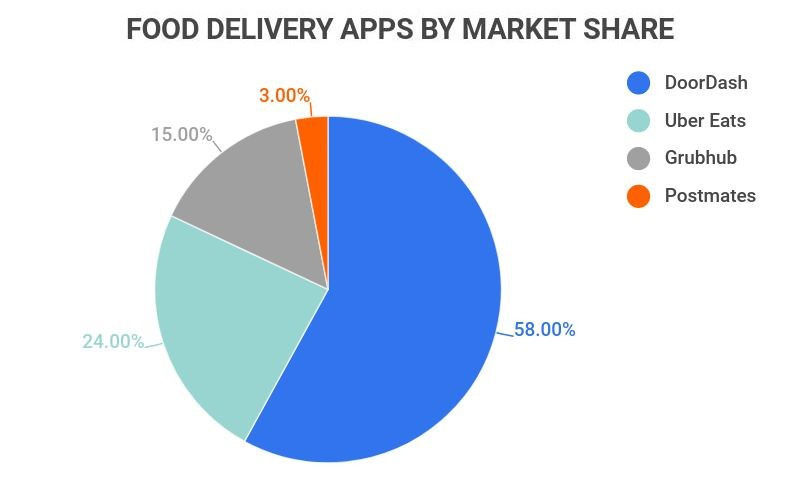
\includegraphics[width=.98\linewidth]{Comps Proposal/Delivery Market.jpeg}
    \caption{
        Saturation of Online Food Delivery Market
    }
    \label{fig:second-page}
\end{figure}

This project will be very useful for the average consumer as it will give them the access to a convenient tool that will save them time and money. This project benefits the average delivery app user as this web will give them the ability to save money on commonly used service other than through coupons or special limited time deals on the apps. However, this web has implications to be potentially detrimental for online food delivery businesses; consumers would reap the benefits of saving money on online food deliveries at the expense of these conglomerates. If this web project were to be expanded so that a consumer could order and pay without having to change apps, then this web could potentially even steer consumers towards specific applications that would offer the best deals, increasing competitions among delivery apps. However, in the limited time for this project, I will focus on the price comparison component rather than a creating dual functioning food delivery and price comparison web.

\begin{figure}
    \centering
    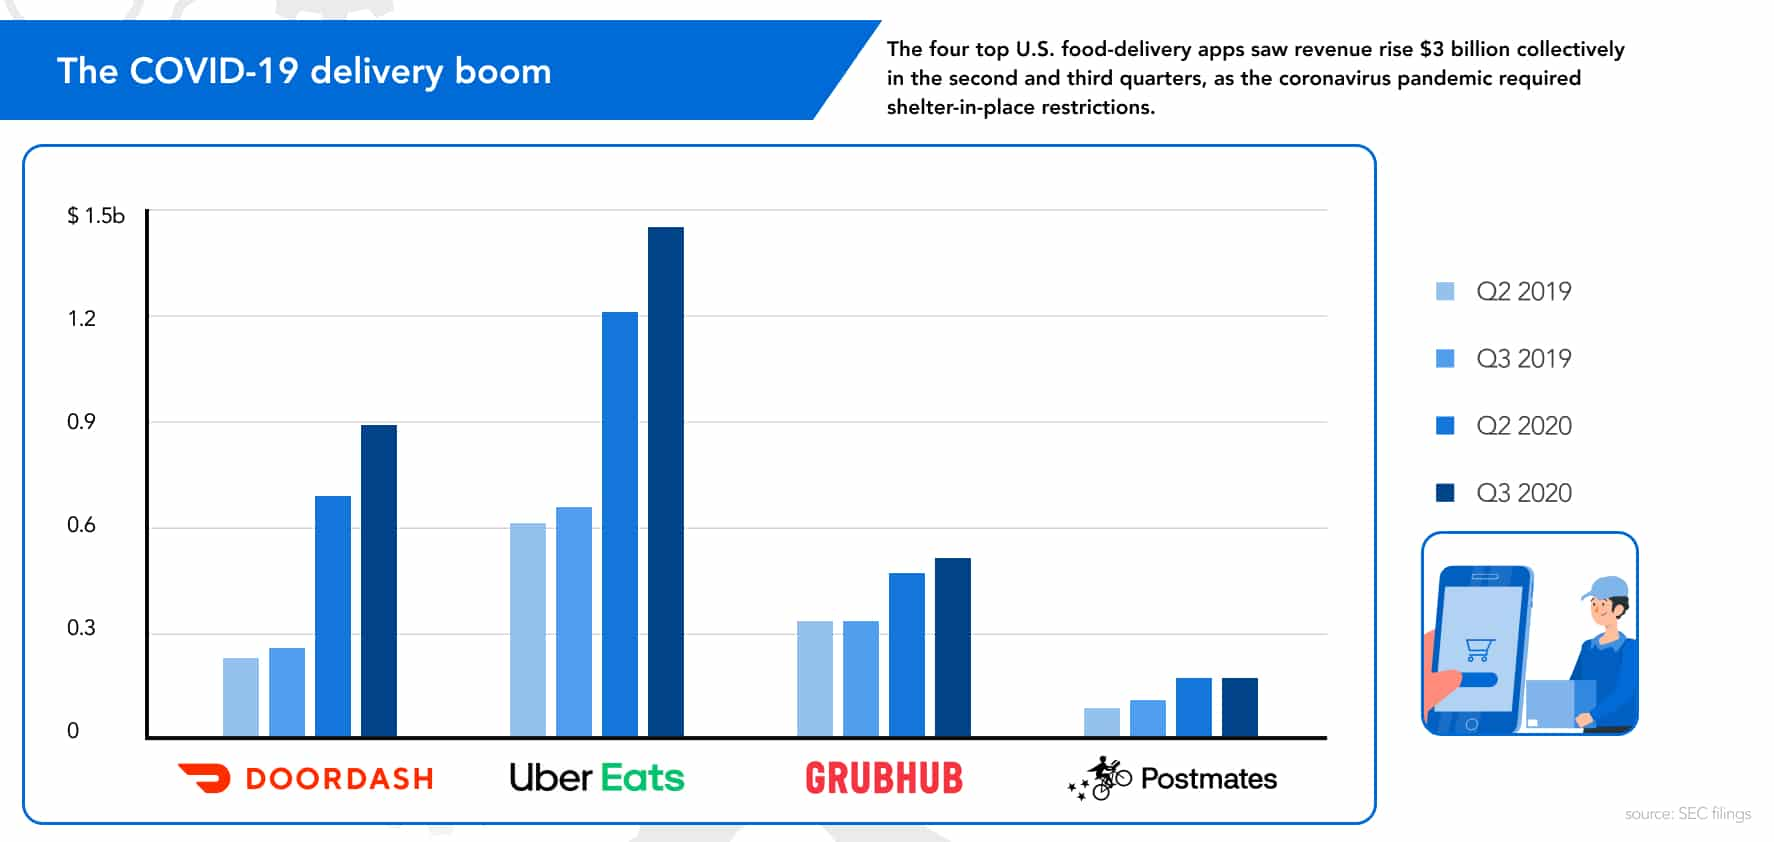
\includegraphics[width=.98\linewidth]{Comps Proposal/Covid.jpeg}
    \caption{
        Financial Effect of Covid-19 on Online Food Delivery
    }
    \label{fig:second-page-1}
\end{figure}  

\section{Technical Background}

For this comprehensive project, the overall stack for the web application is going to be: the user enters the restaurant or food category they want to order from into the web application. Some food categories the user can choose from  can either include a type of cuisine or the type of restaurant, such as "Korean" or "Fast Food" respectively. Then the app finds and lists the respective restaurants within the user's general vicinity. The user selects the restaurant that they want to order from and then web application then presents them the respective menu, from which the user can select what they want in their order. After the user selects all that they want from the menu, the web application will then process this and then outputs a list of the available delivery options for that specific order. At the top of the output screen will the total cost of the order without delivery services and fees accounted for. Below the order cost will be a list of delivery options, which will each contain the title of the company that will deliver the order, the estimated time for delivery, and the additional delivery and service fees.

For this project, the method in which real-time data will be extracted from Uber Eats, Postmates, Grubhub, and DoorDash will be through web scraping. As explained in the article \citetitle{WebScraping}, web scraping is the automated retrieval of data from the text of a web with the aid of bots and storing said data in a structured format. 

With the onset of Covid-19 and the subsequent rapid increase in users of online-to-offline food delivery service, the online food delivery market has become largely saturated. According to \citetitle{Saturation}, there have been both major positive and negative impacts on the online delivery market: the positive effect is that the pandemic has provided a suitable condition for online food delivery companies to promote their services. The negative impact that the pandemic has had on the online food delivery market is that it has triggered "the acceleration of market saturation and reduce the market potential". This has led artificially inflated menu pricing from specific restaurants and the addition of hidden fees and costs to both the restaurants and consumers of the online delivery market.

This project aims to prevent consumers from having to deal with these predatory behaviors from major food delivery app companies by finding them the best deals possible. In doing so, the hope for this project is to potentially reinvigorate a largely saturated market. The convenience of ordering food online has ironically become a hassle in itself for a large number of consumers, especially for those still in school or on a budget. 

\section{Prior Work}

Some prior work that has been done to solve similar issues in the online food delivery market are the delivery price comparison apps “Mealme”  and “FoodBoss”.

Mealme is an iOS app that has features similar to what I want in my web application. A breakdown of MealMe: the iOS app first allows the user to set a specific price range for their desired food delivery order. Next, the app will display multiples lists that fit into the consumer's price range including trending items, daily deals, popular restaurants, cheapest deliverable food and drink options, and so forth, all relative the user's location. One problem with this application is that it is only available on iOS. That is why I plan on creating a web application so that it may be available for all users, as long as they have access to a computer or cell phone. I will not try to emulate all the components of Mealme since the problem in doing that would essentially be me trying to recreate an app that hires hundreds of thousands of dollars worth of coders in salary, within four months. That would become a far too complicated task to complete for the given timeline for this project.

The Mealme claims that the app uses “A.I.” to find the best deals possible for its users, which is not true. What the app does do is it web scrapes data from these major delivery company's apps and presents them in a comprehensible way to its users. However, the app’s interface is not fluid, in that it takes a long time to load, and it occasionally does not display a specific delivery service option for a food order. This leaves room for errors such as longer than expected delivery times, missing orders, and inaccurate delivery fee calculations, such as the negligence of hidden service fees unique to each major delivery app.

Foodboss is essentially the Kayak for food delivery services, in that it compares the delivery prices of nearby restaurants. This application's function is the most similar to what I want to do for this project. However, similar to MealMe, the application is only available on the IPhone whereas I want to create a web that is available to all users.

Though this app is most similar to what I want to emulate, for the given timeline and scope of this project, trying to create a web with all the components of MealMe would be a far too daunting and complicated task to complete.  However, for the timeline of this project, the most reasonable scope would be to build a web application that solely focuses on comparing the total cost of a set online delivery orders from the four major delivery applications. Delivery fees and taxes will be included into the total cost of each delivery app.

\begin{figure}
    \centering
    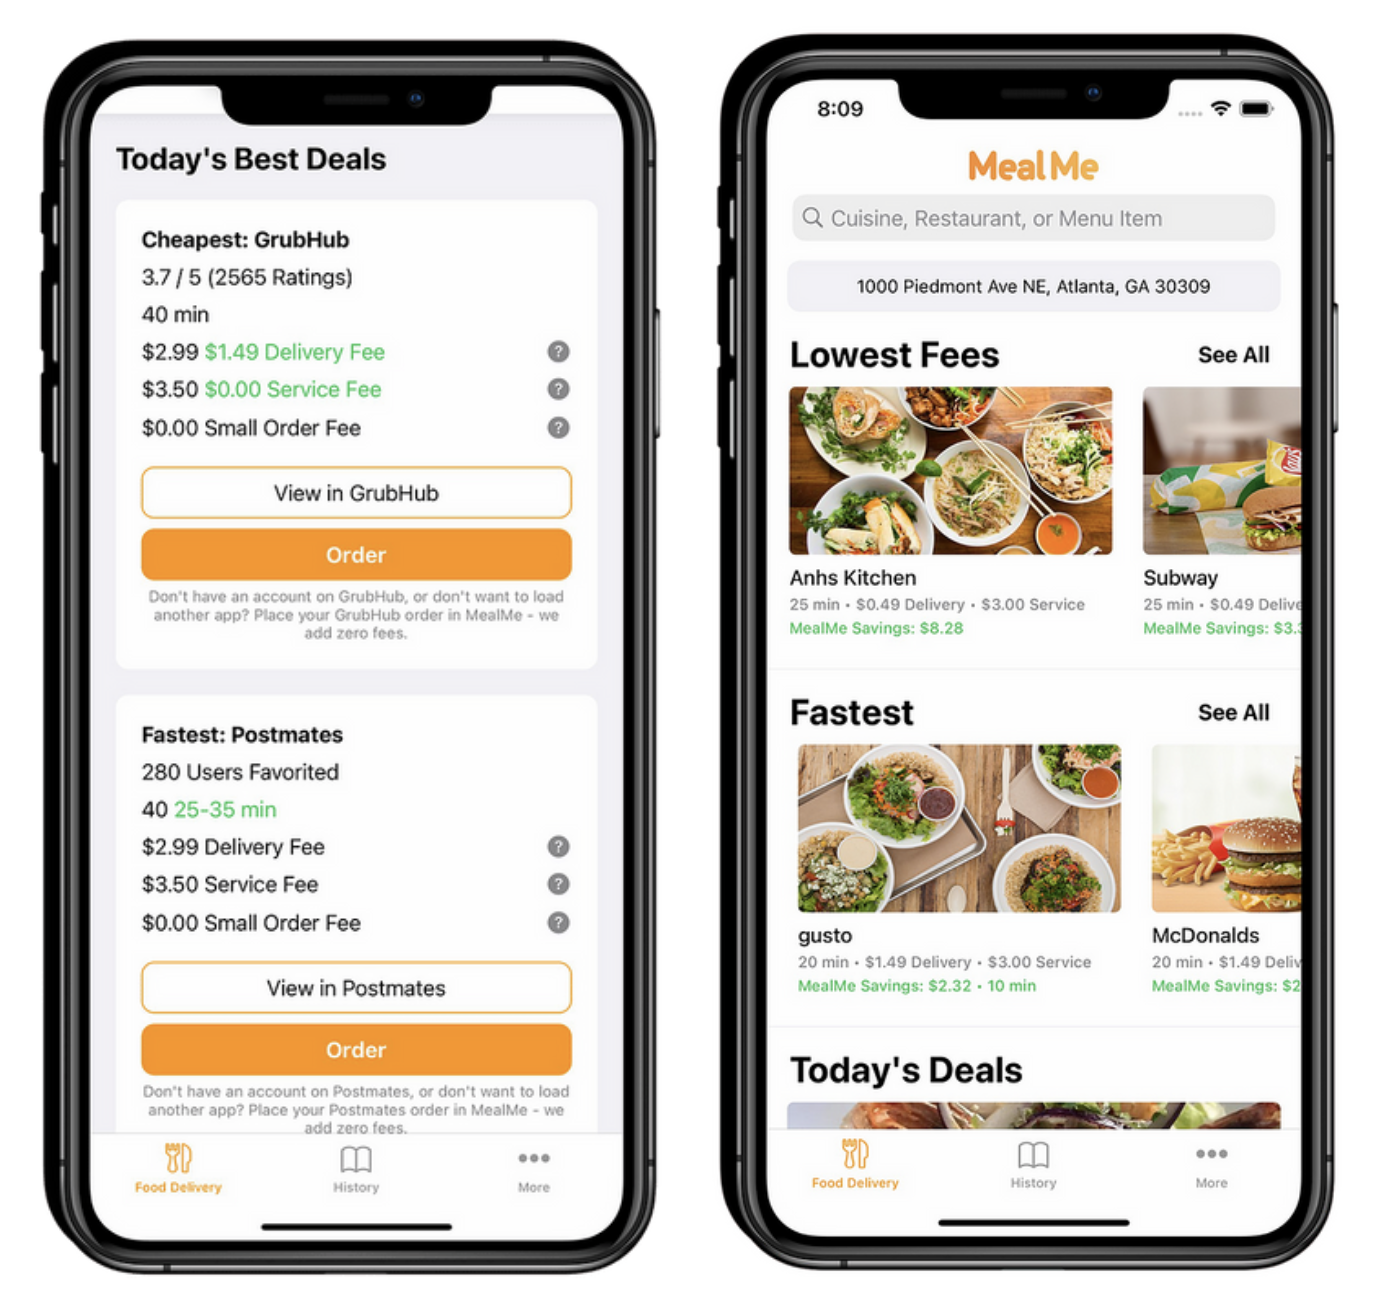
\includegraphics[width=.98\linewidth]{Comps Proposal/Mealme.png}
    \caption{
        MealMe Interface
    }
    \label{fig:second-page-2}
\end{figure}

\section{Methods}

I plan on using Octoparse for this project because this web data extraction tool is free and it also enables users to scrape unstructured data from major applications such as these major food delivery apps. Octoparse can save this data in different formats including Excel, plain text and HTML, which will be necessary for this project. This data scraping and formatting would otherwise be difficult or near impossible within the given time frame of this project. This is because the extraction of data from these major corporation web applications would be impossible without the legal and written consent of these companies. Also, I would need to create my own bots and find a way to illegally extract data from the these major corporation website apps. Though I do not mind ripping off major corporations, for the sake of this project and the amount of time given to complete it, this would be completely impossible and unnecessary.

\begin{figure}
    \centering
    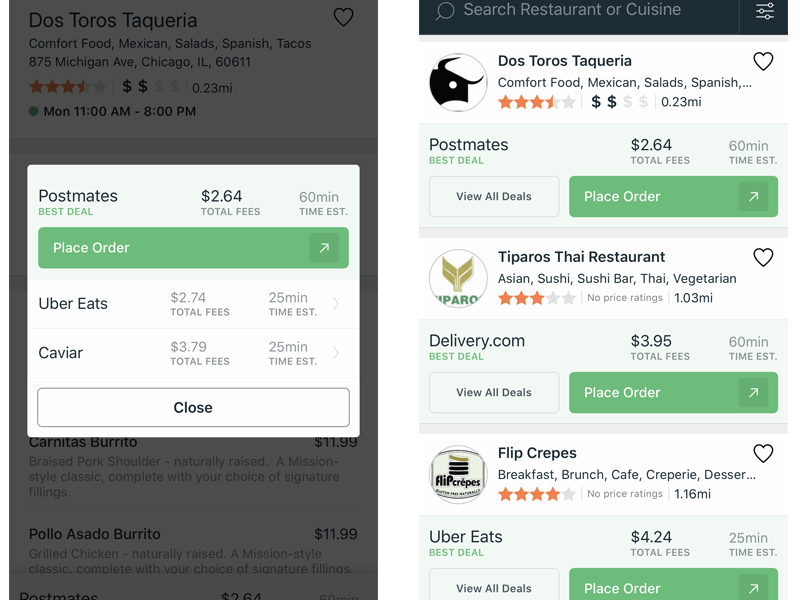
\includegraphics[width=.98\linewidth]{Comps Proposal/FoodBoss.png}
    \caption{
        FoodBoss Interface
    }
    \label{fig:second-page-3}
\end{figure}

For this comprehensive project, since I plan to utilize web scraping to pull real-time data from the Uber Eats, GrubHub, Postmates, and DoorDash, the main application stack for this web application project is: How do I want users to interact with this website? 

The goal for this web application at its core is to give its users the ability to aggregate and compare prices between major food delivery apps. The best way to do this is by designing the web application so that it functions similarly as to how a major food delivery app would.

First, the web application would need to have a search bar for certain restaurants so that the user can search for what they want. Ideally, I would implement an interact-able website interface by using a Yelp plug-in but that's beyond the scope of this project and the allowed timeline. In this web application, when a user searches for a restaurant, the order in which the application should work is:

\begin{enumerate}[label=(\Alph*)]
\item Find nearby restaurants and provide info such as location and general food type after user enters what they want into search bar.
\item Highlight which delivery apps can deliver for that particular restaurant, if any can.
\item Pull up the restaurant's menu and allow the user to select what menu items they want by checking boxes.
\item After the user has selected in their order, the web application will display the total order price and then all of the associated fees itemized for each app.
\item Final cost and total time estimated for order delivery will then be displayed. A box can be checked to show pricing if the user has the any of the apps' premium subscription.
\item If a specific delivery service is not available for that particular restaurant or specific order, then the output on the list will be labeled as "Not Available".
\end{enumerate}

I can aggregate all of this, meaning I will not have to repeat process for each of delivery website. This is only if I can figure out how to work with the data feed. 

Another method that I can follow in order to better understand and utilize web scraping is by following the \citetitle{Ben} by Ben Minor. This comprehensive tutorial on web scraping uses Python which would be a suitable language for this web application since Python has been the leading web scraping language for the better part of a decade. The tutorial uses the Python BeautifulSoup4 library, which is super lightweight, versatile, and makes quick work of web pages with limited used of JavaScript and animation. Beautiful Soup is a library that sits atop an HTML or XML parser, providing Pythonic idioms for iterating, searching, and modifying the parse tree. This tutorial uses Uber Eats as an example which is perfect for this project. However, it may not be as efficient as using Octoparse as it does a better job in aggregating the process of web scraping multiple websites whereas this method requires extra work for the same result.

\begin{figure}
    \centering
    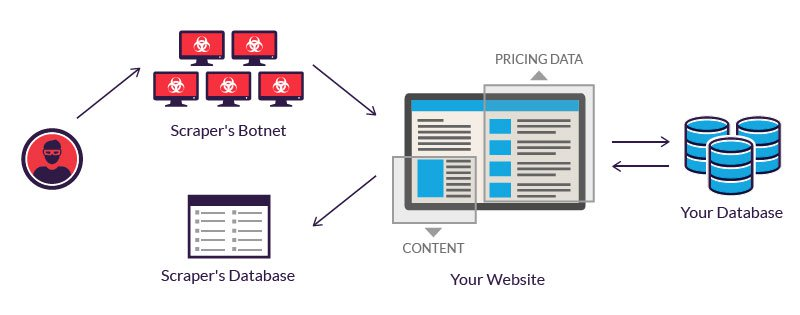
\includegraphics[width=.98\linewidth]{Comps Proposal/What is Scraping.jpeg}
    \caption{
        How Web Scraping Works
    }
    \label{fig:second-page-4}
\end{figure}

\section{Evaluation Metrics}

The main goal in testing this project is to evaluate whether or not this web application functions as intended. The important aspects of this web application worth testing is:

\begin{itemize}
    \item Is the app convenient to use? have beta testers test that)
    \item Is the web application intuitive?
    \item Is the outputted information correct?
    \item Is the output list load time sub-half second?
    \item Are there any abuse cases? Meaning does it work under the corner cases? 
    \subitem Example cases: Uber Eats doesn't exist; user inputs fake restaurant or items; data feeds become corrupted; i.e. anything in which the processing deviates from normal operations
    \item How does the web application handle these deviations? How can they be corrected?
\end{itemize}

The best way to evaluate how well this web application project could save money for potential users is through entering a set number of orders from different restaurants into the web application. Each of the orders will be unique in that they each contain different food items or drinks and that they will be from specific restaurants. Some of the order sets will purposefully contain fake items, an inordinate amount of one item, or items not available at said restaurant.

Another way in which this project will evaluated is through the enlisting of random test users. This will include students from high schools surrounding Occidental College, and students, staff members, and even professors from Occidental College. Since these people are the main demographic for this project, only they would be the most suitable testers to earn feedback from. An important aim for this project is the feeling on convenience and lack of frustration for these users. I do not want this web application to feel as if it is an extra unnecessary step for an action as simple as ordering food through an app. I would consider the web application a failure if and only if it fails to save its users money less than 50\% of the time or if it becomes more of an inconvenience than just checking multiple delivery apps for the best deal.

\begin{figure}
    \centering
    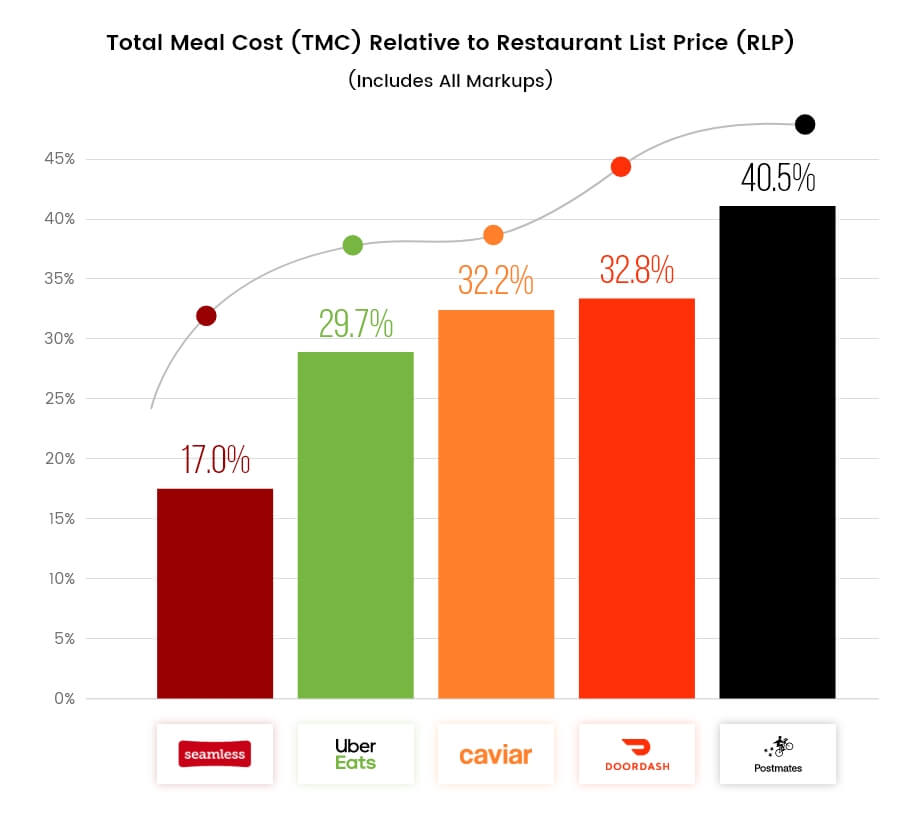
\includegraphics[width=.98\linewidth]{Comps Proposal/TMC.jpeg}
    \caption{
        How Much Extra Customers Pay per App
    }
    \label{fig:second-page-5}
\end{figure}

\section{Ethical Considerations}

According to an article titled \citetitle{Covid}, the impact of the Covid-19 pandemic on the online food delivery market has had both positive and negative consequences: "In the United States, the market has more than doubled during the COVID-19 pandemic, following healthy historical growth of 8 percent". Though the the market for delivery has become popular with the the onset of social distancing, this has also given rise for companies to take advantage of this, leading to potentially ethically ambiguous decisions by the major delivery companies. This includes the artificial inflation of delivery fees and restaurant item costs. This means that ordering a specific item from a restaurant for online delivery is more expensive than if a user were to order in person. The cost of convenience has scaled up online and has been moved into the food delivery market.

This means that delivery fees have been volatile and even differ between each delivery app for the same exact order from a restaurant. If a customer were to order a typical meal from a fast food restaurant say priced around \$25, then the customer total cost (on average) would end up being \$35 as it would also included delivery fees, driver tips, and platform service fees. This is the case for all of the major online food delivery apps in the market. Since customers do not directly see the service commissions that restaurants pay platforms, some restaurants raise their delivery-menu prices to cover this cost, while others opt for pricing consistency, spreading the markup among all customers. Also worth noting is that restaurants themselves receive around only 55 percent of the total customer spend.

According to \citetitle{HiddenFees}, "When you order through a delivery app, you pay multiple parties, including the driver and the companies that offer the apps, like Uber Eats and Postmates. In some cases, you pay the restaurants extra fees as well".
Uber eats mandates a profit-sharing arrangement (Companies cannot opt out of this option unless they have a marketing/business/unique partnership to negate these fees in exchange for something like exclusivity: Chick-fila and DoorDash in Canada: DoorDash offers no kickback if Chickfila exclusively works with DoorDash, same wit) where they assert that Uber Eats existing brings revenue to restaurant s they otherwise would not receive, such that they charge restaurants between 15 and 30\% of the order cost and listing fees. Fees in which restaurants simply pass onto the consumers. Fees that increase the 10\% standard service fee that Uber Eats charges on all of their non-membership orders. Generating a cascading fee hierarchy that is passed almost exclusively to the consumer. 

\section{Proposed Timeline}
For the timeline of my project starting this summer, I have to start thinking about programming the project for my testing users. Below is a list of all the dates for my project and major events that need to happen to fulfill finishing my project on time. 

\begin{itemize}
    \item Aug. 1 - Aug. 14: Configure data feed from third party services to extract data from target delivery companies.
    \item Aug. 15 - Aug. 28: Develop method for processing data feed based on needed queries.
    \item Aug. 29 - Sep. 11: Program site to output desired real-time total order delivery cost with set order from specific restaurant
    \item Sep. 12 - Sep. 25: Make improvements to project code and continue testing
    \item Sep. 26 - Oct. 9: Make sure that varying orders can be used to calculate costs
    \item Oct. 10 - 23: Continue modifying and implementing features into web if time frame allows it
    \item Oct. 24 - Nov. 6: Start outsourcing evaluations for web to demographics such as students and professors from other schools
    \item Nov. 7 - Nov. 20: Continue with user testing and gather feedback to finish incorporating improvements into web application
    \item Nov. 21 - Dec. 4: Finish the final comprehensive project paper and code for web application
 
\end{itemize}

\printbibliography

\end{document}
